\setcounter{chapter}{7-1}

\chapter{Neural Networks 2 - Training Techniques, Regularization}

\setcounter{section}{6}

\section{Optimizing neural network parameters}

    We now understand both how neural networks work, and how to \textbf{train} them. We can use gradient descent to \textbf{optimize} their parameters.
    
    But, we can do better than a simple SGD approach with step size $\eta(t)$. We'll try out some \textbf{modifications} that can speed up our training, and make better models.
    
    \secdiv
    
    \subsection{Mini-batch}
    
        \subsubsection{Review: Gradient Descent Notation}
        
            Let's review some gradient descent notation. We want to \textbf{optimize} our objective function $J$ using $W$.
            
            We do this using the gradient. This gradient depends on our current weights at time $t$, $\blu{W_{t}}$.
            
            \begin{equation}
                \overbrace{
                    \;\;
                    \nabla_W J
                    \;\;
                }^{\text{General Gradient}}
                \quad
                \longrightarrow
                \quad
                \overbrace{
                    \nabla_W J ( \blu{ W_{t} } )
                }^{\text{Gradient at time $t$}}
            \end{equation}
            
            Our update rule is:
            
            \begin{equation}
                \red{ W_{\text{new}} }
                \;\;=\;\;
                \blu{ W_{\text{old}} }
                -
                \eta
                \overbrace{
                    \Big(
                        \nabla_W J ( \blu{ W_{\text{old}} } )
                    \Big)
                }^{\text{Gradient}} 
            \end{equation}
            
            Or, using timestep $t$:
            
            \begin{equation}
                \red{ W_{t+1} } 
                \;\;=\;\;
                \blu{ W_t }
                -
                \eta
                \overbrace{
                    \Big(
                        \nabla_W J ( \blu{ W_t } )
                    \Big)
                }^{\text{Gradient}}
            \end{equation}
            
            What is our objective function $J$? Without regularization, it's based on our loss function. We can get loss for each of our data points:
                \note{We won't define $J$ here, because it is slightly different for SGD and BGD. We'll get to that below.}
            
            \begin{equation}
                \ex{\loss}{i}
                =
                \overbrace{
                    \loss(
                    \; \ex{g}{i} \;
                    ,\eyi
                    )
                }^{\text{Loss for data point $i$}}
            \end{equation}
            
            Our guess $\ex{g}{i}$ depends on both our current data point $\exi$, and the current weights $\blu{ W_t }$:
            
            \begin{equation}
                \ex{\loss}{i}(\blu{ W_t })
                \;\;=\;\;
                \loss(
                \;\;
                \overbrace{
                     h(\exi;\blu{ W_t }) 
                }^{\ex{g}{i}}
                \;\;
                ,\eyi
                )
            \end{equation}
    
        \subsecdiv
    
        \subsubsection{Review: BGD vs. SGD}
        
            Let's review our two main types of gradient descent, using the equation
            
            \begin{equation}
                \red{ W_{t+1} } 
                \;\;=\;\;
                \blu{ W_t }
                -
                \eta
                \overbrace{
                    \Big(
                        \nabla_W J ( \blu{ W_t } )
                    \Big)
                }^{\text{Gradient}}
            \end{equation}
            
            First, we have \textbf{batch gradient descent}, where we use our \textbf{whole} training set each time we take a step.\\
            
            \begin{definition}
                \vocab{Batch Gradient Descent (BGD)} is a form of gradient descent where we get the \gren{gradient} of our loss function using \purp{all of our training data}.
                
                \begin{equation*}
                    \nabla_W J ( \blu{ W_t } )
                    \;\;=\;\;
                    \sum_{i=1}^n
                    \;\;
                    \overbrace{
                        \nabla_W
                        \Big(
                            \ex{\loss}{i}(\blu{ W_t })
                        \Big)
                    }^{\text{Each data point}}
                \end{equation*}
                
                We get the gradient for each data point, and then \purp{add} all of those gradients up. We use this \purp{combined gradient} to take \gren{one step}.
                
                We \gren{repeat} this process every time we want to take a new step.
            \end{definition}
            
            Then, we have \textbf{stochastic gradient descent}, where we use only \textbf{one} data point for each step we take.\\
            
            \begin{definition}
                \vocab{Stochastic Gradient Descent (SGD)} is a form of gradient descent where we get the \gren{gradient} of our loss function using \purp{one data point at a time}.
                
                \begin{equation*}
                    \nabla_W J ( \blu{ W_t } )
                    \;\;
                    =
                    \;\;
                    \overbrace{
                    \nabla_W
                    \Big(
                        \ex{\loss}{i}(\blu{ W_t })
                    \Big)
                    }^{\text{One data point}}
                \end{equation*}
                
                We \purp{randomly} choose one data point $(\exi,\eyi)$ and get the \purp{gradient}. Based on this one gradient, we take our \gren{step}.
                
                For each step, we choose a new \purp{random} data point.
            \end{definition}
            
            These two approaches have tradeoffs:\\
            
            \begin{concept}
                There are \vocab{tradeoffs} between \vocab{SGD} and \vocab{BGD}:
                
                \begin{itemize}
                    \item Each step is \purp{faster} in \purp{SGD} because it only needs to get the gradient for one data point.
                        \begin{itemize}
                            \item Meanwhile, \gren{BGD} is \gren{slower}: each step takes a lot more computation, because we have to get many gradients.
                        \end{itemize}
                        
                    \item Because \gren{BGD} is using all the data, it has a much more \gren{accurate} gradient.
                        \begin{itemize}
                            \item \purp{SGD} often needs much \purp{smaller} steps, because each gradient is less accurate: based on less data.
                        \end{itemize}
                        
                    \item \purp{SGD} \purp{randomly} chooses data points: this random noise can make it harder to overfit.
                        \begin{itemize}
                            \item \gren{BGD} uses all of the data, so we don't reduce overfitting.
                        \end{itemize}
                \end{itemize}
            \end{concept}
        
        \subsecdiv
        
        \subsubsection{Mini-batch}
        
            Rather than picking one or the other, one might think, "why do we have to pick \textbf{every} data point or \textbf{one} data point? Couldn't we pick only a \textbf{few}?"
            
            This is the premise of \textbf{mini-batch}: instead of making a batch out of the entire training set, we \textbf{randomly} select a few data points, and use that as our batch.\\
            
            \begin{definition}
                \vocab{Mini-batch} is a way to \purp{compromise} between SGD and BGD.
                
                To create a mini-batch, we \purp{randomly} select $K$ data points from our training data. 
                
                We treat this mini-batch the same way we would a regular \gren{batch}: get the \purp{gradient} of each data point, \gren{add} those gradients, and take one  step of gradient descent.
                
                \begin{equation*}
                    \nabla_W J ( \blu{ W_t } )
                    =
                    \overbrace{
                        \sum_{i=1}^K
                    }^{K \text{ data points in a mini-batch}} 
                    \nabla_W
                    \Big(
                        \ex{\loss}{i}(\blu{ W_t })
                    \Big)
                \end{equation*}
                
                We gather a \gren{new} mini-batch for each step we want to take.
            \end{definition}
            
            Mini-batch is the \textbf{default} used in most modern packages: it gives us more \textbf{control} over our algorithm, and can often find the \textbf{best} of both worlds.\\
            
            \begin{concept}
                \vocab{Mini-batch} has a lot of benefits of both SGD and BGD:
                
                \begin{itemize}
                    \item Steps are \purp{faster} than BGD: we only need to get the gradient for $K$ points.
                        \begin{itemize}
                            \item The speed no longer \gren{depends} on the total training data size (more data, more gradients): instead, it depends on our batch size $K$.
                        \end{itemize}
                        
                    \item Steps are more \purp{accurate} than SGD: with multiple points, we can get a more stable \gren{gradient}.
                        \begin{itemize}
                            \item This means we can take \purp{bigger} steps.
                        \end{itemize}
                    
                    \item Our batches are \purp{randomly} chosen, like SGD: this can reduce overfitting and avoid shallow local minima.
                \end{itemize}
                
                One more important benefit:
                
                \begin{itemize}
                    \item If we find that a particular problem is better suited for something closer to BGD or SGD, we can \gren{adjust} our batch size $K$.
                        \begin{itemize}
                            \item This gives us more \purp{control} over our learning algorithm.
                        \end{itemize}
                \end{itemize}
            \end{concept}
        
    \secdiv
    
    \subsection{Adaptive Step Size - Challenges}
    
        We now move away from thinking about SGD vs BGD, and instead, we set our sights on improving our \textbf{step size}.
        
        Step size $\eta$ is a difficult problem:
        
        \begin{itemize}
            \item If $\eta$ is \textbf{small}, then our training can take a long \textbf{time}.
            
            \item If $\eta$ is too \textbf{large}, we might \textbf{diverge}: our answer gets way too large.
            
            \item A \textbf{large} step size might also cause \textbf{oscillation}: most of our step is wasted going back and forth, so we go \textbf{slowly} again.
        \end{itemize}
        
        SGD and mini-batch have another problem:
        
        \begin{itemize}
            \item In order to \textbf{converge} according to our theorems (see chapter 3), the step size $\eta(t)$ has to be \textbf{decreasing} in a certain way.
                \note{Check chapter 3 for the exact requirements of the theorem.}
        \end{itemize}
    
    \secdiv
    
    \subsection{Vanishing/Exploding Gradient}
    
        Now, neural networks have one more \textbf{problem}, that we haven't had to deal with before: \textbf{deep} neural networks can cause a problem called "\textbf{exploding/vanishing gradient}".
            \note{By "deep", we just mean "many layers".}
        
        Here's an example: suppose you have a long chain rule, with 8 terms. Our chain rule gets \textbf{longer} with more layers, because each layer needs its own derivatives.
        
        \begin{equation}
            \pderiv{A}{H}
            \;\;=\;\;
            \pderiv{A}{B}
            \cdot
            \pderiv{B}{C}
            \cdot
            \Big(
            \cdots
            \Big)
            \cdot
            \pderiv{G}{H}
        \end{equation}
        
        This chain rule gets \textbf{longer} as we move "\textbf{backwards}" through our network, so the chain rule is longest for the "\textbf{early}" layers: $\ell=1, 2,$ and so on.
        
        Suppose all of our derivatives are roughly $.1$. What happens when we multiply them \textbf{together}?
        
        \begin{equation}
            \pderiv{A}{H}
            \;\; = \;\;
            .1 \cdot .1 \cdot 
            \Big(
            \cdots
            \Big)
            \cdot 
            .1
            \;\; = \;\;
            10^{-8}
        \end{equation}
        
        The derivative becomes really, really small! This is the case of the \textbf{vanishing} gradient: if our gradients are less than one, then as we append more layers, they multiply to get smaller and smaller.
        
        This is a problem: if our gradients in our earlier layers become too \textbf{small}, we'll never make any progress! They'll hardly change.\\
        
        \begin{definition}
            \vocab{Vanishing gradient} is when a deep neural network ends up with \purp{very small gradients} in the \gren{earlier} layers. 
            
            This happens because a deeper neural network has a \gren{longer chain rule}: if all of the terms are \purp{less than one}, they'll multiply into a very small value, "\vocab{vanishing}".
            
            This means that our gradient descent will have \purp{almost no effect} on these earlier weights, \gren{slowing down} our algorithm considerably.
        \end{definition}
        
        What if the gradients are larger than 1? Let's say our derivatives are 10 each.
        
        \begin{equation}
            \pderiv{A}{H}
            = 
            10 \cdot 10 \cdot 
            \Big(
            \cdots
            \Big)
            \cdot 
            10
            =
            10^{8}
        \end{equation}
        
        Now, the early derivatives are becoming \textbf{huge}! This is the case of \textbf{exploding} gradient: if our gradients are greater than one, then as we add layers, they multiply to get bigger.
        
        This is also a problem: we don't want to take \textbf{huge} steps, or we will \textbf{diverge}, or \textbf{oscillate}, and jump huge distances across the \textbf{hypothesis space}.\\
        
        \begin{definition}
            \vocab{Exploding gradient} is when a deep neural network ends up with \purp{very large gradients} in the \gren{earlier} layers. 
            
            This happens because a deeper neural network has a \gren{longer chain rule}: if all of the terms are much \purp{greater than one}, they'll multiply into a very large value, "\vocab{exploding}".
            
            This means that our gradient descent will take \purp{huge steps} in the hypothesis space. This can cause us to \gren{diverge}, miss local minima, or \gren{oscillate}.
        \end{definition}
        
        So, to avoid this, we can't just blindly multiply our gradients and keep a fixed step size.
        
        The solution? Each \textbf{weight} gets its own step size $\eta$.\\
        
        \begin{concept}
            In order to avoid \vocab{vanishing/exploding} gradient problems, we give each \gren{weight} in our network its own \purp{step size} $\eta$.
            
            This allows us to \purp{adjust} the step size for some weights more than others: if our gradient is too large or small, we can fix it.
        \end{concept}
    \secdiv
    
    \subsection{Momentum}
    
        \subsubsection{Solving Oscillation}
    
            Let's look at one common problem we have with gradient descent: \textbf{oscillation}. 
            
            \begin{figure}[H]
                \centering
                    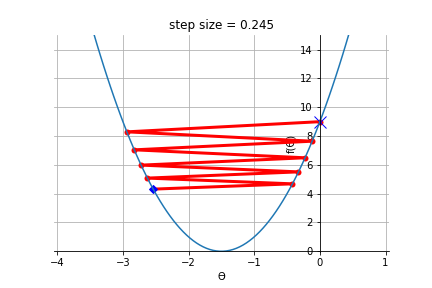
\includegraphics[width=70mm,scale=0.5]{images/gradient_descent_images/oscillate.png}
            \end{figure}
            
            We overshoot our target, and then have to take another step that \textbf{undoes} most of what happened in the previous step. So, we waste a lot of time correcting the last step.
                \note{For example, our first two steps land us in almost the same place we started!}
                
            This can significantly \textbf{slow} down how quickly we converge.
                
            \begin{figure}[H]
                \centering
                    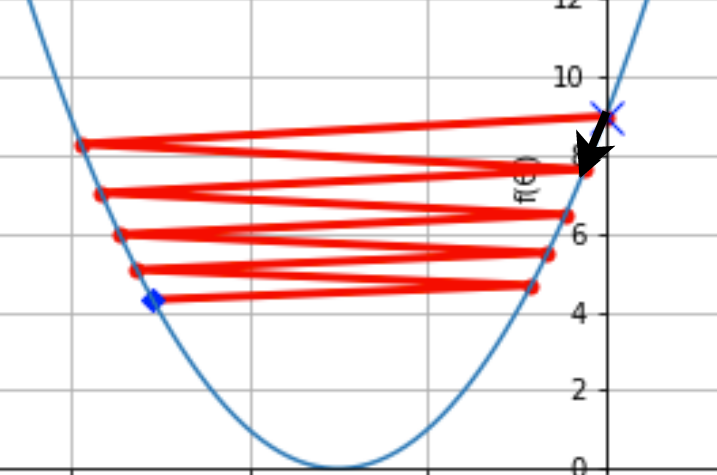
\includegraphics[width=70mm,scale=0.5]{images/nn_2_images/oscillate_zoom.png}
                
                \caption*{The black arrow shows the combined effect of our first two steps: almost nothing!}
            \end{figure}
            
            We don't want to waste time, so we want to remove the "part" of the gradient that is likely to \textbf{cancel} out. 
            
            The \textbf{next} gradient cancels out some of the previous. Our first two steps add up, or "\textbf{average} out" to a small improvement.
            
            If our steps are effectively "averaging", we'll speed up that process: we'll average together the gradients \textit{before} taking our step!
                \note{This means we can take a bigger step in a direction we won't have to cancel!}\\
                
            \begin{concept}
                Since our gradient descent steps \gren{combine} to give us our new model, we can think of them as adding, or "\purp{averaging}" to a more accurate improvement.
            \end{concept}
            
                \note{The only real difference between adding and averaging is whether we divide by the number of terms.}
            
            When our function \textbf{oscillates}, we get the same pattern \textbf{multiple} times: past steps indicate the sort of pattern we'll see in \textbf{future} steps. 
            
            So, we'll average our current gradient with past gradients: that way, the \textbf{component} that gets cancelled out is \textbf{removed}, and we won't have to undo our mistake over and over.\\
            
            \begin{concept}
                \vocab{Oscillation} causes us to move back and forth over the same region \purp{multiple} times, where each step mostly \gren{cancels} out the last.
                
                One solution is to \purp{average out} multiple of our gradients: the part that is "\gren{cancelled} out" should be eliminated by the average.
                
                So, we average our \gren{past} gradients (past oscillation) with our \gren{current} gradient, so we move in a more \purp{efficient} direction, speeding up our algorithm.
            \end{concept}
            
            Another way to think about it: when we \textbf{average} out our current and previous gradient, we're cancelling out what they "\textbf{disagree}" on, and keeping what they \textbf{agree} on.
            
            So, we're taking a step in the direction that multiple gradients agree will \textbf{improve} our model!
            
        
        \subsecdiv
            
        \subsubsection{Weighted averages}
        
            We could naively average all of our gradients \textbf{equally}. But, this would be a bad idea:
            
            \begin{itemize}
                \item It doesn't give you as much control of the algorithm: what if we care more about the \textbf{present} gradient, than the previous one?
                \item Gradients further in the past are \textbf{less likely} to matter: we've moved further away from those positions.
                    \begin{itemize}
                        \item We also need to \textbf{scale} them down, so they don't take up most of the average.
                            \note{If you're averaging 100 terms, and you add one more... it's not going to change much.}
                    \end{itemize}
            \end{itemize}
            
            The first problem is easy to solve: we'll \textbf{weigh} each of our terms differently.\\
            
            \begin{concept}
                A \vocab{weighted average} is used when we want some terms to affect our \purp{average} more than others.
                
                We represent this with \gren{weights}: each weight represents the \purp{proportion} of our average from that term.
                
                \begin{equation*}
                    \text{Weighted Average} =
                    x_1w_1 + x_2w_2 + \dots + x_nw_n
                \end{equation*}
            \end{concept}
            
            \miniex If $w_1=\red{.6}$, that means \red{60\%} of the average comes from $x_1$.
            
            Note that, since we're talking about \textbf{proportions}, they need to add to 1: it wouldn't make sense to have more than 100\% of the average.
            
            At each time step, we're adding one new gradient: the \textbf{present} one.
            
            We'll simplify our average to those two terms: the \textbf{present} gradient, versus all the \textbf{past} gradients.
            
            \begin{itemize}
                \item We represent the importance (\textbf{weight}) of our \textbf{past} gradients using the variable $\red{\gamma}$.
                
                \item We want the two terms to add to 1: so, the importance of \textbf{current} gradient is $\blu{1-\gamma}$.
            \end{itemize}
            
            \begin{equation}
                \overbrace{
                    A_t 
                }^{\text{Average}}
                =
                \overbrace{
                    \red{\gamma} G_{t-1}
                }^{\text{Old gradients}}
                + 
                \overbrace{
                    \blu{(1-\gamma)} g_{t}
                }^{\text{New gradient}}
            \end{equation}
            
            Now, we have \textbf{control} over how much the present or past gradient matters: we just have to adjust $\gamma$. 
            
        \subsecdiv
        
        \subsubsection{Running Average}
        
            We still have some work to do: first, we haven't made it clear how we're incorporating our old gradients: we lumped them into one term.
            
            Let's try building up from $t=1$. We'll assume our previous gradients are 0, for simplicity.
            
            \begin{equation}
                A_0=g_0=0
            \end{equation}
            
            Our first step will average this with our \textbf{first} gradient:
            
            \begin{equation}
                A_1 
                =  
                \red{\gamma} g_0 + \blu{(1-\gamma)} g_1
            \end{equation}
            
            Simplifying to:
            
            \begin{equation}
                A_1 =  \blu{(1-\gamma)} g_1
            \end{equation}
            
            What about our second step? 
            
            \begin{equation}
                A_2
                =
                \overbrace{
                    \red{\gamma} G_{t-1}
                }^{\text{Old gradients}}
                + 
                \blu{(1-\gamma)} g_2
            \end{equation}
            
            We \textit{could} just plug in $g_1$. But, $A_1$ contains the information about our first gradient $g_1$, \textbf{and} the gradient before it, $g_0$.
            
            \begin{equation}
                A_2
                =
                \overbrace{
                    \red{\gamma} A_1
                }^{\text{Contains $g_1$, $g_0$}}
                + 
                \blu{(1-\gamma)} g_2
            \end{equation}
            
            We can repeat this process:
            
            \begin{equation}
                A_3 = 
                \overbrace{
                    \red{\gamma} A_{2}
                }^{\text{Contains $g_2$,$g_1$, $g_0$}}
                + 
                \overbrace{
                    \blu{(1-\gamma)} g_3
                }^{\text{New gradient}}
            \end{equation}
            
            
            
            
            

        
        
        
        
        
        
        
\section{Chatgpt attempt}

    \subsection{Adjustable Step Sizes}

\subsubsection{Running Averages}
\index{adjustable step sizes!running average}
Let's begin with the concept of a \textit{running average}, which is a computational approach for approximating a possibly weighted average of a series of data. Consider our data sequence to be $a_1, a_2, \ldots$; we then establish a sequence of running average values, $A_0, A_1, A_2, \ldots$, using the following equations:
\begin{align*}
A_0 &= 0 \
A_t &= \gamma_t A_{t-1} + (1 - \gamma_t) a_t
\end{align*}
where $\gamma_t \in (0, 1)$. If $\gamma_t$ remains constant, this results in a \textit{moving} average, expressed as:
\begin{align*}
A_T & = \gamma A_{T-1} + (1 - \gamma) a_T \
& = \gamma (\gamma A_{T-2} + (1 - \gamma) a_{T-1}) + (1 - \gamma) a_T \
& = \sum_{t = 1}^T \gamma^{T-t}(1 - \gamma) a_t
\end{align*}
Hence, it is evident that the $a_t$ values closer to the end of the sequence $T$ have a greater impact on $A_T$ than earlier values.

On the other hand, if we set $\gamma_t = (t - 1) / t$, we obtain the actual average.
\question{
Verify the previous statement on your own.
}

\subsubsection{Momentum}
\index{adjustable step sizes!momentum}
We can now employ techniques similar to running averages to outline strategies for determining $\eta$. The simplest method, \textit{momentum}, involves averaging recent gradient updates to remove the component of motion that oscillates back and forth in a specific direction. For momentum, we have:
\begin{align*}
V_0 & = 0 \
V_t & = \gamma V_{t-1} + \eta \nabla_W J(W_{t-1}) \
W_t & = W_{t-1} - V_t
\end{align*}
Although this does not precisely resemble an adjustable step size, if we let $\eta = \eta'(1 - \gamma)$, the rule appears identical to performing an update with step size $\eta'$ on a moving average of the gradients with parameter $\gamma$:
\begin{align*}
M_0 & = 0 \
M_t & = \gamma M_{t-1} + (1 - \gamma) \nabla_W J(W_{t-1}) \
W_t & = W_{t-1} - \eta' M_t
\end{align*}
\question{Prove to yourself that these formulations are equivalent.}

In this case, $V_t$ will be larger in dimensions that consistently have the same sign for $\nabla_{W}$ and smaller for those that do not. Although we now have \textit{two} parameters to set ($\eta$ and $\gamma$), the expectation is that the algorithm will deliver better overall performance, justifying the effort to find suitable values for them. Often, $\gamma$ is set to around $0.9$.

\question{Would momentum have more or less of an effect if you set $\gamma = 0.1$ compared to setting it to $0.9$?}

\subsubsection{Adadelta}
\index{adjustable step sizes!adadelta}
Another valuable idea is to take larger steps in areas where $J(W)$ is nearly flat (since there is no risk of taking an excessively large step due to a high gradient) and smaller steps when the surface is steep. We will apply this idea independently to each weight, resulting in a method called \textit{adadelta}, which is a variant of \textit{adagrad} (for adaptive gradient). Although our weights are indexed by layer, input unit, and output unit, for simplicity, let $W_j$ represent any weight in the network (the same process will be applied to all of them).
\begin{align*}
g_{t,j} & = \nabla_W J(W_{t-1})j \
G{t,j} & = \gamma G_{t - 1,j} + (1 - \gamma)g_{t,j}^2 \
W_{t,j} & = W_{t-1, j} - \frac{\eta}{\sqrt{G_{t,j} + \epsilon}}g_{t,j}
\end{align*}
The sequence $G_{t,j}$ is a moving average of the square of the $j$th component of the gradient. We square it to be insensitive to the sign—we want to determine whether the magnitude is large or small. Then, we perform a gradient update to weight $j$, dividing the step size by $\sqrt{G_{t,j} + \epsilon}$, which is larger when the surface is steeper in direction $j$ at point $W_{t-1}$ in weight space. As a result, the step size will be smaller when the surface is steep and larger when it is flat.

\section{Old Materials}

\section{Optimizing neural network parameters}
\label{sec:make_nn_work}




\subsection{Adaptive step-size}



\subsubsection{Running averages}
\index{adaptive step size!running average}
We'll start by looking at the notion of a {\em running average}.  It's
a computational strategy for estimating a possibly weighted average of
a sequence  of data.  Let our data sequence be $a_1, a_2, \ldots$;
then we define a sequence of running average values, $A_0, A_1, A_2,
\ldots$ using the equations
\begin{align*}
A_0 &= 0 \\
A_t &=  \gamma_t A_{t-1} +  (1 - \gamma_t) a_t
\end{align*}
where $\gamma_t \in (0, 1)$.  If $\gamma_t$ is a constant, then this
is a {\em  moving} average, in which 
\begin{align*}
A_T & = \gamma A_{T-1} + (1  - \gamma) a_T \\
& = \gamma (\gamma A_{T-2} + (1  - \gamma) a_{T-1}) + (1  - \gamma) a_T \\
& = \sum_{t = 1}^T \gamma^{T-t}(1 - \gamma) a_t
\end{align*}
So, you can see that inputs $a_t$ closer to the end of the sequence $T$
have  more effect on $A_T$ than early inputs.

If, instead, we set $\gamma_t = (t - 1)  / t$, then we get the actual
average.
\question{
Prove to yourself that the previous assertion holds.
}
% \begin{align*}
% A_1 &= a_1\\
% A_2 &= \frac{1}{2}A_1 + \frac{1}{2}a_2 = \frac{1}{2}(a_1 + a_2)\\
% A_3 &= \frac{2}{3}A_2 + \frac{1}{3}a_3 = \frac{2}{3} \cdot \frac{1}{2}(a_1 + a_2) + \frac{1}{3}a_3 = \frac{1}{3}(a_1 + a_2 + a_3)
% \end{align*}

\subsubsection{Momentum} \index{adaptive step size!momentum}
Now, we can use methods that are a bit like running averages to
describe strategies for computing $\eta$.
The simplest method is {\em momentum}, in  which we try to ``average'' recent
gradient updates,  so that if they have been bouncing back and forth
in some direction, we take out that component of the motion.  For
momentum, we have
\begin{align*}
V_0 & = 0 \\
V_t & = \gamma V_{t-1} + \eta \nabla_W J(W_{t-1}) \\
W_t & = W_{t-1} - V_t
\end{align*}
This doesn't quite look like an adaptive step size.  But what we can
see is that, if we let $\eta = \eta'(1 - \gamma)$, then the rule looks exactly like doing an update with
step size $\eta'$ on a moving average of the gradients with parameter
$\gamma$:
\begin{align*}
M_0 & = 0 \\
M_t & = \gamma M_{t-1} + (1 - \gamma) \nabla_W J(W_{t-1}) \\
W_t & = W_{t-1} - \eta' M_t
\end{align*}
\question{Prove to yourself that these formulations are equivalent.}


We will find that $V_t$ will be bigger in dimensions that consistently
have the same sign for $\nabla_{W}$ and smaller for those that
don't.   Of course we now have {\em two}  parameters  to set ($\eta$
and $\gamma$), but the
hope is  that the algorithm will perform better overall, so it will be
worth trying to find good values for them.  Often $\gamma$ is  set to
be something like $0.9$.  
\begin{examplebox}
\begin{center}
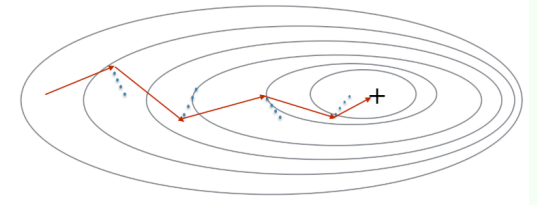
\includegraphics[scale=0.7]{figures/momentum.png}
\end{center}
The red arrows show the update after each successive step of
mini-batch gradient descent with momentum.  The blue points show the
direction of the gradient with respect to the mini-batch at each step.
Momentum smooths the path taken towards the local minimum and leads to
faster convergence.
\end{examplebox}
\question{If you set $\gamma = 0.1$, would momentum have more of an
  effect or less of an effect than if you set it to $0.9$?
}

\subsubsection{Adadelta}\index{adaptive step size!adadelta}
Another useful idea is this:  we would like to take larger steps in
parts of the space where $J(W)$ is nearly flat (because there's no risk of
taking too big a step due to the gradient being large) and smaller
steps when it is steep.  We'll apply this idea to each weight
independently, and end up with a method called {\em adadelta}, which
is a variant on {\em adagrad} (for
adaptive gradient).   Even though our weights are indexed by layer,
input unit and output unit,  for simplicity here,  just let $W_j$ be
any weight in the network (we will do the same thing for all of
them).   
\begin{align*}
 g_{t,j} & = \nabla_W J(W_{t-1})_j \\
 G_{t,j} & = \gamma G_{t - 1,j} + (1 - \gamma)g_{t,j}^2 \\
W_{t,j} & = W_{t-1, j} - \frac{\eta}{\sqrt{G_{t,j} + \epsilon}}g_{t,j} 
\end{align*}
The sequence $G_{t,j}$ is a moving average of the  square of the
$j$th component of the gradient.  We square it in order to be
insensitive to the sign---we want to know whether the magnitude is big
or small.  Then, we perform a gradient update to weight $j$, but
divide the step  size by $\sqrt{G_{t,j} + \epsilon}$, which is larger
when the surface is steeper in direction $j$ at point $W_{t-1}$ in
weight space;  this means that the step size will be smaller when it's
steep and  larger when it's flat.

\subsubsection{Adam}\index{adaptive step size!adam}

Adam has become the default method of managing step sizes in neural
networks\note{Although,  interestingly, it may actually violate the
  convergence conditions of {\sc sgd}: {\scriptsize\tt
    arxiv.org/abs/1705.08292}}.   It combines the ideas  of
momentum and adadelta.  We start by writing moving averages of the
gradient and squared gradient, which reflect estimates of the mean and
variance of the gradient for weight $j$:
\begin{align*}
 g_{t,j} & = \nabla_W J(W_{t-1})_j \\
 m_{t,j} & = B_1m_{t - 1,j} + (1 - B_1)g_{t,j} \\
 v_{t,j} & = B_2v_{t - 1,j} + (1 - B_2)g_{t,j}^2  \;\;.
\end{align*}

A problem with these estimates is that, if we initialize $m_0 = v_0 = 0$,
they will always be biased (slightly too small).  So we will correct
for that bias  by defining
\begin{align*}
 \hat{m}_{t,j} & = \frac{m_{t,j}}{1 - B^t_1}  \\
 \hat{v}_{t,j} & = \frac{v_{t,j}}{1 - B^t_2}  \\
 W_{t,j} & = W_{t-1,j} - \frac{\eta}{\sqrt{\hat{v}_{t,j} +
    \epsilon}}\hat{m}_{t,j} \;\;.
\end{align*}
Note that $B^t_1$ is $B_1$ raised to the power $t$, and likewise for
$B^t_2$.  To justify these corrections, note that if we were to expand $m_{t,j}$
in terms of $m_{0,j}$ and $g_{0,j}, g_{1,j}, \dots, g_{t,j}$ the coefficients would
sum to $1$.  However, the coefficient behind $m_{0,j}$ is $B_1^t$ and since 
$m_{0,j} = 0$, the sum of coefficients of non-zero terms is $1 - B_1^t$, hence
the correction.  The same justification holds for $v_{t,j}$.

Now, our update for weight $j$ has a step size that takes the
steepness into account, as in adadelta, but also tends to move in the
same direction, as in momentum.  The authors of this method propose
setting $B_1 = 0.9, B_2 = 0.999, \epsilon = 10^{-8}$.  Although we now
have even more parameters, Adam is not highly sensitive to their values
(small changes do not have a huge effect on the result).
\question{Define $\hat{m_j}$ directly as a moving average of
  $g_{t,j}$.  What is the decay ($\gamma$ parameter)?
}
Even though we now have a step-size for each weight, and we have to
update various quantities on each iteration of gradient descent, it's
relatively easy to implement by maintaining a matrix for each quantity
($ m^{\ell}_t, v^{\ell}_t, g^{\ell}_t, {g^{2}_t}^{\ell} $) in each
layer of the network. 

\section{Regularization}\index{neural network!regularization}
So far, we have only considered optimizing loss on the training data
as our objective for neural network training.   But, as we have
discussed before, there is a risk of overfitting if we do this.  The
pragmatic fact is that,  in current deep neural networks, which tend to be very
large and to be trained with a large amount of data,  overfitting is
not a huge problem.  This runs counter to our current theoretical
understanding and the study of this question is a hot area of
research.  Nonetheless, there are several strategies for regularizing
a neural network, and they can sometimes be important.

\subsection{Methods related to ridge regression}

One group of strategies can, interestingly, be shown to have similar
effects to each other: early stopping, weight decay, and adding noise
to the training data. \note{Result is due to Bishop, described in his
  textbook and here {\tt\scriptsize doi.org/10.1162/ neco.1995.7.1.108}.}

Early stopping is the easiest to implement and is in fairly common
use.  The idea is to train on your training set, but at every {\em
  epoch} (a pass through the whole training set, or possibly more
frequently), evaluate the loss of the current $W$ on a {\em validation
  set}.  It will generally be the case that the loss on the training
set goes down fairly consistently with each iteration, the loss on the
validation set will initially decrease, but then begin to increase
again.  Once you see that the validation loss is systematically
increasing, you can stop training and return the weights that had the
lowest validation error.

Another common strategy is to simply penalize the norm of all the
weights, as we did in ridge regression.  This  method is known as {\em
  weight decay}\index{neural network!weight decay}, because when we take the gradient of the objective
$$ J(W) = \sum_{i = 1}^{n}\mathcal{L}(\text{NN}(x^{(i)}), y^{(i)}; W)
+ \lambda\|W\|^2 $$ 
we end up  with an update of the form
\begin{align*}
 W_t &= W_{t-1} -
       \eta\left(\left(\nabla_{W}\mathcal{L}(\text{NN}(x^{(i)}),
       y^{(i)}; W_{t-1})\right) + 2\lambda W_{t-1}\right)\\ 
& = W_{t-1}(1 - 2\lambda\eta) - \eta\left(\nabla_{W}\mathcal{L}(\text{NN}(x^{(i)}),
       y^{(i)}; W_{t-1})\right) \;\;.
\end{align*}
This rule has the form of first ``decaying'' $W_{t-1}$ by a factor of
$(1 - 2 \lambda \eta)$ and then taking a gradient step.  

Finally, the same effect can be achieved by perturbing the $\ex{x}{i}$
values of the training data by adding a small amount of zero-mean
normally distributed noise before each gradient computation.  It makes
intuitive sense that it would be more difficult for the network to
overfit to particular training data if they are changed slightly on
each training step.

\subsection{Dropout}
Dropout\index{neural network!dropout} is a regularization method that was designed to work with deep
neural networks.  The idea behind it is, rather than perturbing the
data every time we train, we'll perturb the network!  We'll do this by
randomly, on each training step, selecting a set of units in each
layer and prohibiting them from participating.   Thus, all of the
units will have to take a kind of  ``collective'' responsibility for
getting the answer right, and will not be able to rely on any small
subset of the weights to do all the necessary computation.  This tends
also to make the network more robust to data perturbations.

During the training phase, for each training example, for each unit,
randomly with probability $p$ temporarily set $a^{\ell}_j = 0$. There
will be no contribution to the output and no gradient update for the
associated unit.
\question{
Be sure you understand why, when using {\sc sgd}, setting an
activation value to 0 will cause that unit's weights not to be updated
on that iteration. 
}

When we are done training and want to use the network to make
predictions, we multiply all weights by $p$ to achieve the same average
activation levels. 

Implementing dropout is easy!  In the forward pass during training, we let
$$ a^{\ell} = f(z^{\ell}) * d^{\ell} $$
where $*$ denotes component-wise product and $d^{\ell}$ is a vector of
$0$'s and $1$'s drawn randomly with probability $p$.  
The backwards pass depends on $a^{\ell}$, so we do not need to make
any further changes to the algorithm.

It is common to set $p$ to $0.5$, but this is something one might
experiment with to get good results on your problem and data.

% Dropout is no longer in common use, but it is still interesting to
% think about.

\subsection{Batch Normalization}

Another strategy that seems to help with regularization and robustness
in training is {\em batch normalization}.  \index{neural network!batch normalization}
\note{For more  details see {\tt\scriptsize arxiv.org/abs/1502.03167}.}
It was originally
developed to address a problem of {\em covariate shift}:  that is, if
you consider the second layer of a two-layer neural network, the
distribution of its input values is changing over time as the first
layer's  weights change.  Learning when the input distribution is
changing is extra difficult:  you have to change your weights to
improve your predictions, but also just to compensate for a change in
your inputs  (imagine, for instance, that the magnitude of the inputs
to your layer is increasing over time---then your weights will have to
decrease, just to keep your predictions the same).

So, when training with mini-batches, the idea is to {\em standardize}
the input values for each mini-batch, just in the way that we did it
in Section~\ref{realFeatures} of Chapter~\ref{chap:features}, subtracting off the mean
and dividing by the standard deviation of each input dimension.  This
means that the scale of the inputs to each layer remains the same, no
matter how the weights in previous layers change.  However, this
somewhat complicates matters, because the computation of the weight
updates will need to take into account that we are performing this
transformation.  In the modular view, batch normalization can be seen
as a module that is applied to $z^l$, interposed after the product
with $W^l$ and before input to $f^l$.\note{We follow here the
suggestion from the original paper of applying batch normalization
before the activation function.  Since then it has been shown that,
in some cases, applying it after works a bit better. But there
aren't any definite findings on which works better and when.}

Although batch-norm was originally justified based on the problem of
covariate shift, it's not clear that that is actually why it seems to
improve performance.  
Batch normalization can also end up having a regularizing effect for similar
reasons that adding noise and dropout do:  each mini-batch of data
ends up being mildly perturbed, which prevents the network from
exploiting very particular values of the data points.

Let's think of the batch-norm layer as taking $Z^l$ as input and
producing an output $\widehat{Z}^l$ as output.  But now, instead of
thinking of $Z^l$ as an $n^l \times 1$ vector, we have to explicitly
think about handling a mini-batch of data of size $K$, all at once, so
$Z^l$ will be $n^l \times K$, and so will the output $\widehat{Z}^l$.  

Our first step will be to compute the {\em batchwise} mean and
standard deviation.  Let $\mu^l$ be the $n^l \times 1$ vector where
\[\mu^l_i = \frac{1}{K} \sum_{j = 1}^K Z^l_{ij}\;\;,\]
and let $\sigma^l$ be the $n^l \times 1$ vector where 
\[\sigma^l_i = \sqrt{\frac{1}{K} \sum_{j = 1}^K (Z^l_{ij} - \mu_i)^2}\;\;.\]

The basic normalized version of our data would be a matrix, 
element $(i, j)$ of which is 
\[\overline{Z}^l_{ij} = \frac{Z^l_{ij} - \mu^l_i}{\sigma^l_i + \epsilon}\;\;,\]
where $\epsilon$ is a very small constant to guard against division by
zero. 
However, if we let these be our $\widehat{Z}^l$ values, we really are
forcing something too strong on our data---our goal was to normalize
across the data batch, but not necessarily force the output values to
have exactly mean 0 and standard deviation 1.  So, we will give the
layer the ``opportunity'' to shift and scale the outputs by adding new
weights to the layer.  These weights are $G^l$ and $B^l$, each of
which is an $n^l \times 1$ vector.  Using the weights, we define the
final output to be 
\[\widehat{Z}^l_{ij} = G^l_i \overline{Z}^l_{ij} + B^l_i\;\;.\] 
That's the forward pass.  Whew!

Now, for the backward pass, we have to do two things:  given
$\partial L / \partial \widehat{Z}^l$, 
\begin{itemize}
\item Compute $\partial L / \partial Z^l$ for back-propagation, and
\item Compute $\partial L / \partial G^l$ and $\partial L / \partial
  B^l$ for gradient updates of the weights in this layer.
\end{itemize}

Schematically\note{For simplicity we will drop the reference to the layer $l$ in the rest of the derivation}
\[\frac{\partial L}{\partial B} = \frac{\partial L}{\partial
    \widehat{Z}}\frac{\partial \widehat{Z}}{\partial B}\;\;.\]
It's hard to think about these derivatives in matrix terms, so we'll
see how it works for the components.  
$B_i$ contributes to $\widehat{Z}_{ij}$ for all data points $j$ in the
batch.  So
\begin{align*}
  \frac{\partial L}{\partial B_i} & =
                     \sum_j \frac{\partial L}{\partial \widehat{Z}_{ij}}
                     \frac{\partial \widehat{Z}_{ij}}{\partial B_i} \\
                                  & = \sum_j \frac{\partial L}{\partial \widehat{Z}_{ij}}\;\;,
                                    \end{align*}
Similarly, $G_i$ contributes to $\widehat{Z}_{ij}$ for all data points
$j$ in the batch.  So
\begin{align*}
  \frac{\partial L}{\partial G_i} & =
                     \sum_j \frac{\partial L}{\partial \widehat{Z}_{ij}}
                     \frac{\partial \widehat{Z}_{ij}}{\partial G_i} \\
             & =  \sum_j \frac{\partial L}{\partial \widehat{Z}_{ij}} \overline{Z}_{ij}\;\;.
\end{align*}
Now, let's figure out how to do backprop.  We can start schematically:
\[\frac{\partial L}{\partial Z} = \frac{\partial L}{\partial \widehat{Z}}
                               \frac{\partial \widehat{Z}}{\partial Z}\;\;.\]
And because dependencies only exist across the batch, but not across
the unit outputs, 
\[\frac{\partial L}{\partial Z_{ij}} =
  \sum_{k=1}^K\frac{\partial L}{\partial \widehat{Z}_{ik}}
                            \frac{\partial \widehat{Z}_{ik}}{\partial Z_{ij}}\;\;.\]
The next step is to note that
\begin{align*}                          
\frac{\partial \widehat{Z}_{ik}}{\partial Z_{ij}} &=
  \frac{\partial \widehat{Z}_{ik}}{\partial \overline{Z}_{ik}}
  \frac{\partial \overline{Z}_{ik}}{\partial Z_{ij}} \\
&= G_i \frac{\partial \overline{Z}_{ik}}{\partial Z_{ij}}\;\;.
\end{align*}                          
And now that
\[
\frac{\partial \overline{Z}_{ik}}{\partial Z_{ij}}  = 
\left(\delta_{jk} - \frac{\partial \mu_i}{\partial Z_{ij}}\right) \frac{1}{\sigma_i} -
\frac{Z_{ik} - \mu_i}{\sigma_i^2} \frac{\partial \sigma_i}{\partial Z_{ij}} \;\;,
\]
where $\delta_{jk} = 1$ if $j = k$ and $\delta_{jk} = 0$ otherwise.
Getting close!  We need two more small parts:
\begin{align*}
  \frac{\partial \mu_i}{\partial Z_{ij}} & = \frac{1}{K} \;,\\
  \frac{\partial \sigma_i}{\partial Z_{ij}} & = 
        \frac{Z_{ij} - \mu_i}{K \sigma_i}\;\;.
\end{align*}
Putting the whole crazy thing together, we get
\[\frac{\partial L}{\partial Z_{ij}} =
  \sum_{k=1}^K\frac{\partial L}{\partial \widehat{Z}_{ik}}
  G_i\frac{1}{K \sigma_i}\left(\delta_{jk}K-1 - \frac{(Z_{ik} - \mu_i)(Z_{ij} - \mu_i)}{\sigma_i^2}
\right)\;\;.
\]


%%% Local Variables:
%%% mode: latex
%%% TeX-master: "top"
%%% End:
